\label{ch:sdc}

\section{SDC Overview}

Spectral deferred corrections (SDC) is an iterative scheme used to integrate
the thermodynamic variables, $(\rho X_k,\rho h)$, over a time step.  It has
been shown to be more accurate and efficient than Strang splitting in a
terrestrial, non-stratified, low Mach number reacting flow solver \cite{Non11},
so we would like to develop an SDC version of \maestro.

\maestro\ integrates the following system of equations:
\begin{eqnarray}
\frac{\partial\Ub}{\partial t} &=& 
    -\Ub\cdot\nabla\Ub  - \frac{1}{\rho}\nabla\pi 
    - \frac{\rho-\rho_0}{\rho} g\eb_r,\label{eq:momentum}\\
\frac{\partial(\rho X_k)}{\partial t} &=& 
    -\nabla\cdot(\rho X_k\Ub) + \rho\omegadot_k,\label{eq:species}\\
\frac{\partial(\rho h)}{\partial t} &=& 
    -\nabla\cdot(\rho h\Ub) + \frac{Dp_0}{Dt} 
    + \rho\Hnuc + \nabla\cdot k_{\rm th}\nabla T,\label{eq:enthalpy}
\end{eqnarray}
together with base state evolution equations and a constraint equation.
By default, \maestro\ advances the thermodynamic variables by coupling
the different physical processes together (advection, diffusion, reactions) using
Strang splitting.  Specifically, we integrate the reaction terms 
over half a time step ignoring contributions from advection and diffusion,
then from this intermediate state we integrate the advection and diffusion terms over
a full time step (while ignoring reactions), and finally
integrate the reactions over a half time step (ignoring advection and diffusion).
For problems where
the reactions and/or diffusion greatly alter the energy balance or composition 
as compared to advection, this operator splitting approach can lead to large 
splitting errors and highly inaccurate solutions.
This issue is can be particularly exasperating 
for low Mach number methods that can take large advection-based time steps.

An alternate approach to advancing the thermodynamic variables is SDC. 
SDC is an iterative approach to couple the various processes
together, with each process seeing an 
approximation of the other processes as a source term.  The SDC
algorithm converges to an integral representation of the solution in
time that couples all of the processes together in a self-consistent
fashion, see \cite{Non11}.

As a first attempt, we will work on coupling advection and reactions only
via SDC, with a base state that is fixed in time, but not space.

\section{Strang-Splitting Without Thermal Diffusion or Base State Evolution}

In the Strang splitting version of \maestro, the reaction and advection
processes operate independent of one-another.  The species and
enthalpy equations are integrated over $\Delta t$ using the following
sequence:

\begin{itemize}

\item React for $\Delta t/2$:

In the Strang splitting version of \maestro, the reaction network solves just
the reaction portion of the species evolution equations along with a
temperature evolution equation.  This is done using a standard stiff ODE solver
package (like {\tt VODE}) on the system:
\begin{eqnarray}
\frac{dX_k}{dt} &=& \omegadot_k(\rho,X_k,T), \\
\frac{dT}{dt}   &=& 
    \frac{1}{c_p} \left ( -\sum_k \xi_k  \omegadot_k  + \Hnuc \right ).
\end{eqnarray}
Here, $T$ is evolved solely to evaluate the reaction rates,
$\omegadot_k(\rho,X_k,T)$.  Furthermore, we simplify the problem
``freezing'' the thermodynamics---i.e., $c_p$ and $\xi_k$ are evaluated at the
start of the integration and held constant thereafter.
The density remains constant during this step, i.e., 
$\rho^\mathrm{new} = \rho^\mathrm{old}$, and we
update the enthalpy at the end of the integration as:
\begin{equation}
h^\mathrm{new} = h^\mathrm{old} + \frac{\Delta t}{2} \Hnuc.
\end{equation}

\item Advect for $\Delta t$:

Beginning with the results from the previous reaction half time step, we integrate
that state using the equations
\begin{eqnarray}
\frac{\partial(\rho X_k)}{\partial t} &=& 
    -\nabla\cdot(\rho X_k\Ub), \\
\frac{\partial(\rho h)}{\partial t} &=& 
    -\nabla\cdot(\rho h\Ub) + \frac{Dp_0}{Dt}.
\end{eqnarray}
Note that no reaction terms appear here.  Since the advection
takes place using the state updated from the reaction step, the effect
of the reactions is implicitly contained in the advective update.

\item React for $\Delta t/2$:

Finally, we react again, starting with the state left by the advection
step.

\end{itemize}

Note that \maestro\ uses a predictor-corrector approach.  After integrating $(\rho X_k,\rho h)$ over
the time step, we use this time-advanced state to get a better estimate of a time-centered $\beta_0$
and $S$.  We re-compute the advective velocities using an updated divergence constraint and repeat 
the thermodynamic variable advance.

\section{SDC Without Thermal Diffusion or Base State Evolution}
In the SDC version, the {\tt VODE} integration at the end of an SDC
iteration is responsible for updating all the thermodynamic quantities
including both the advection (incorporated via a piecewise constant advective 
flux divergence source term) and the reactions.  This provides a much stronger coupling between
the physical processes.  In particular, our system now looks like:
\begin{eqnarray}
\frac{d(\rho X_k)}{dt} &=& \rho \omegadot_k(\rho,X_k,T) - \underbrace{\nabla\cdot(\rho X_k\Ub)}_{A_{\rho X_k}}\label{eq:sdc:rhoX} \\
\frac{d(\rho h)}{dt}   &=& \rho \Hnuc - \underbrace{\nabla\cdot(\rho h\Ub) + \frac{Dp_0}{Dt}}_{A_{\rho h}} \label{eq:sdc:rhoh}
\end{eqnarray}
Here, $A_{\rho X_k}$ and $A_{\rho h}$ are piecewise-constant (in time)
approximations to the change in ${\rho X_k}$ and ${\rho h}$ (respectively)
due to the advection.  These are constructed by calling {\tt density\_advance}
and {\tt enthalpy\_advance} in \maestro\ and passed into the network solver
during the reaction step.  A flowchart of the \maestro\ SDC algorithm is 
shown in figure~\ref{fig:sdc:flowchart}.

\begin{figure}[tb]
\centering
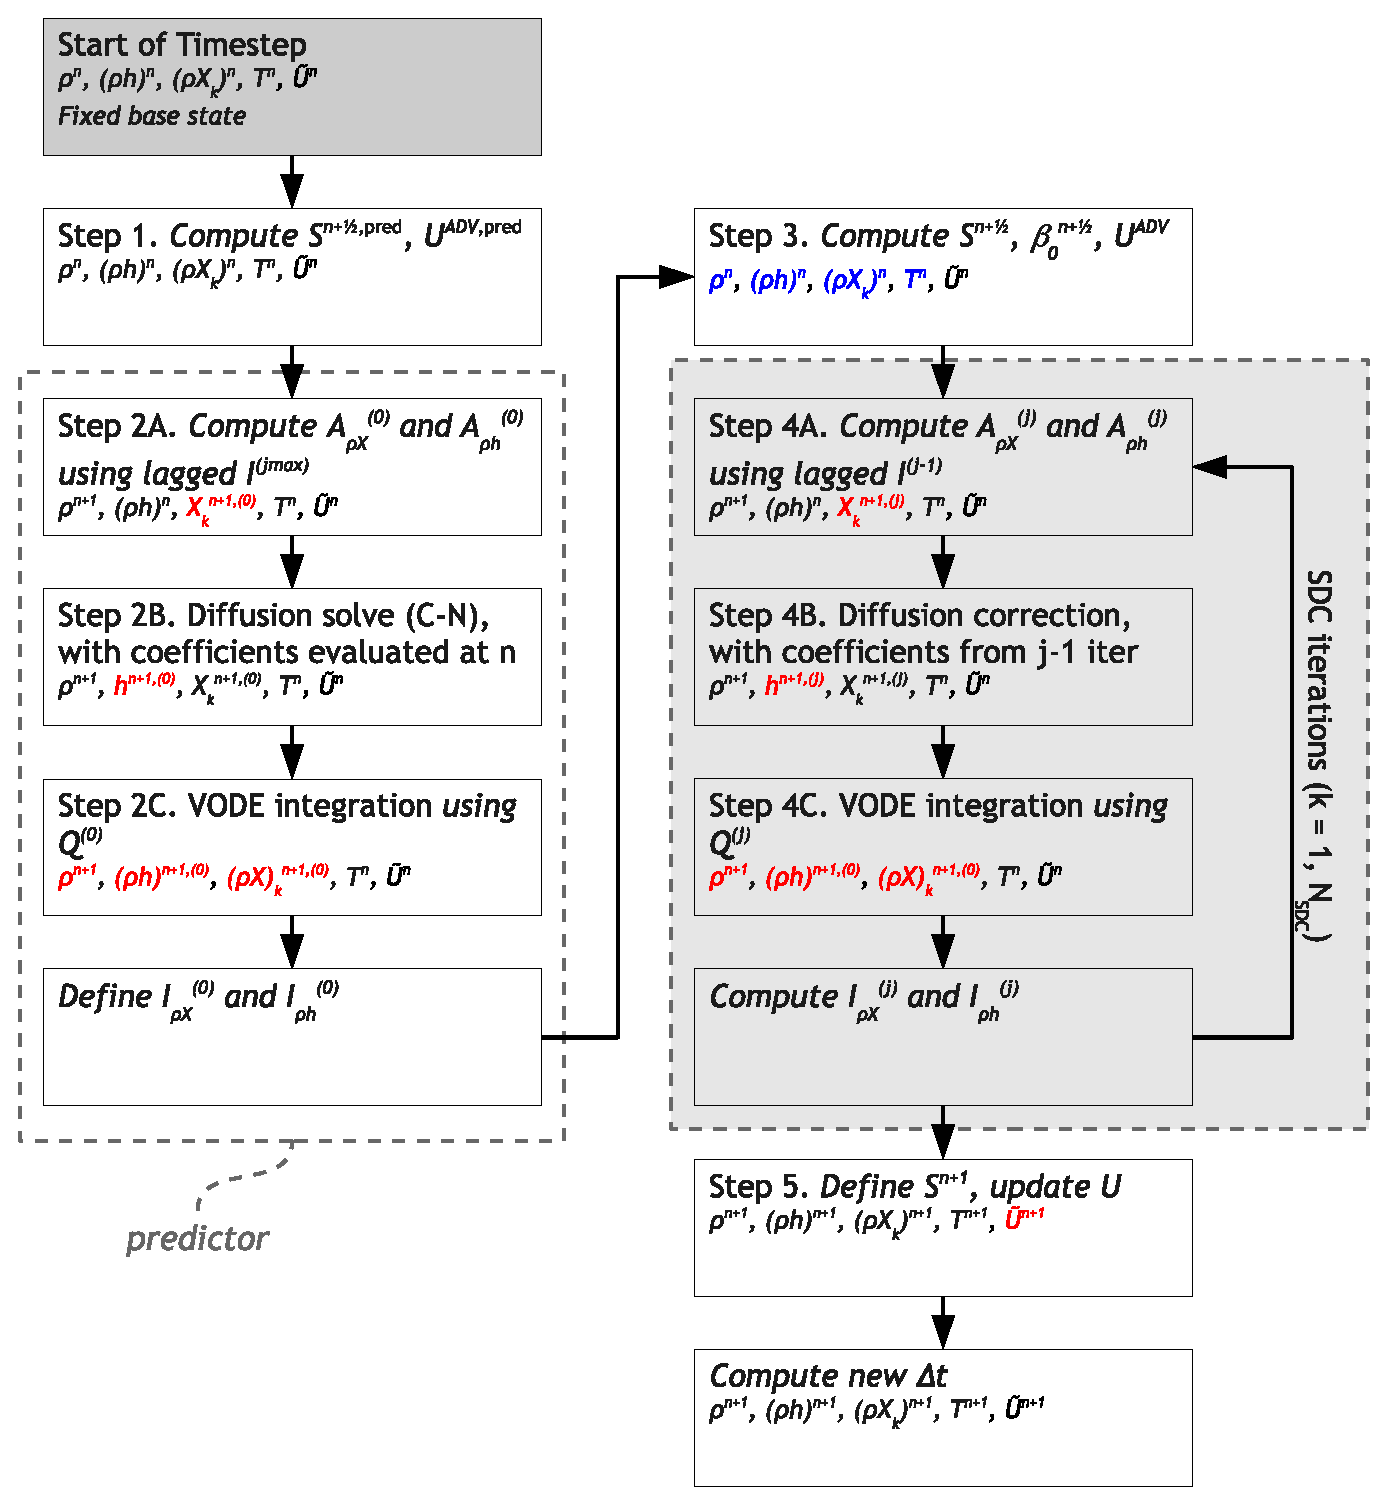
\includegraphics[scale=0.65]{\sdcfigpath/flowchart_SDC}
\caption[Graphical flowchart of \maestro\ SDC]
  {\label{fig:sdc:flowchart} A flowchart of the \maestro\ SDC algorithm.  The
  thermodynamic state variables and local velocity are
  indicated in each step.  The base state is not shown as it is time-independent.
  Red text indicates that quantity was
  updated during that step.  The predictor is 
  outlined by the dotted box.  The blue text indicates state
  variables that are the same in {\bf Step 6} as they are in
  {\bf Step 2}, i.e., they are unchanged by the predictor steps.
  The SDC loop is shown in the gray dotted box.}
\end{figure}


\subsection{Advective Update}

In the advective update, our goal is to compute $A_{\rho X_k}$ and
$A_{\rho h}$.  These terms approximate the following:
\begin{eqnarray}
A_{\rho X_k} &=&  \left [- \nabla \cdot (\rho X_k \Ub) \right ]^{n+1/2} \\
A_{\rho h}   &=&  \left [- \nabla \cdot (\rho h \Ub) + \frac{Dp_0}{Dt} \right ]^{n+1/2}
\end{eqnarray}
The construction of the interface states used in the advective terms
uses either a time-lagged or iteratively-lagged approximation to the reaction
terms ($I_{\rho X_k}$ and $I_{\rho h}$, see below) as a source term in the interface
prediction.  This explicitly couples the reaction process to the
advection process.


\subsection{Final Update}

The RHS routine that the ODE solver operates on will first construct
the density as:
\begin{equation}
\rho = \sum_k (\rho X_k)
\end{equation}
It will then derive the temperature from the equation of state.  If we
are running with {\tt use\_tfromp = T}, then we do
\begin{equation}
T = T(\rho, p_0, X_k)
\end{equation}
otherwise, we do
\begin{equation}
T = T(\rho, h, X_k)
\end{equation}
Note that in contrast to the Strang splitting version, here we call the EOS
every time we enter the RHS routine, but here we call the EOS to compute temperature
rather than thermodynamic coefficients.

Finally we integrate the ODE system (Eqs.~\ref{eq:sdc:rhoX} and \ref{eq:sdc:rhoh}).
At the end of the integration, we define $I_{\rho X_k}$ and $I_{\rho h}$.  The actual 
form of these depends on what quantities we predict to edges during 
the construction of the advective fluxes.
Note that we only need $I_{\rho X_k}$ and $I_{\rho h}$ for the
prediction of the interface states, and not the {\tt VODE} integration.
This is because all we need from the advection solver is the
approximation to $A_{\rho X_k}$ and $A_{\rho h}$ and not the final
updated state.

\subsection{Species Source Terms.}
For the species prediction, the form of $I$ depends on
{\tt species\_pred\_type} (see \S \ref{sec:pred:density}).
We note that there is no $I$ term for $\rho$ or $\rho'$ prediction, since
the density evolution equation does not have a reaction source term.
\begin{itemize}
\item {\tt species\_pred\_type} = 1 ({\tt predict\_rhoprime\_and\_X})
or 3 ({\tt predict\_rho\_and\_X})

\begin{equation}
I_{X_k} = \frac{1}{\rho^{n+\myhalf}} \left [ 
      \frac{(\rho X_k)^\mathrm{new} - 
            (\rho X_k)^\mathrm{old}}{\Delta t} - A_{\rho X_k}  \right ].
\end{equation}
(Andy's Idea) Define $I_{X_k}$ using
\begin{equation}
I_{X_k} = \frac{X_k^\mathrm{new} - X_k^\mathrm{old}}{\Delta t} - A_{X_k},
\end{equation}
where we first define a state that has only been updated with advection:
\begin{equation}
\frac{(\rho X_k)^{(1)} - (\rho X_k)^\mathrm{old}}{\Delta t} = A_{\rho X_k},
\end{equation}
and then define the species mass fractions,
\begin{equation}
X_k^{(1)} = (\rho X_k)^{(1)} / \sum_k (\rho X_k)^{(1)}, \quad 
X_k^\mathrm{old} = (\rho X_k)^\mathrm{old} / \sum_k (\rho X_k)^\mathrm{old}, \quad 
X_k^\mathrm{new} = (\rho X_k)^\mathrm{new} / \sum_k (\rho X_k)^\mathrm{new},
\end{equation}
and finally define $A_{X_k}$ using
\begin{equation}
\frac{X^{(1)} - X^\mathrm{old}}{\Delta t}= A_{X_k}.
\end{equation}
\item {\tt species\_pred\_type} = 2 ({\tt predict\_rhoX})
\begin{equation}
I_{\rho X_k} = \frac{(\rho X_k)^\mathrm{new} - (\rho X_k)^\mathrm{old}}{\Delta t} - A_{\rho X_k}.
\label{eq:sdc:Irhoo}
\end{equation}
\end{itemize}

\subsection{Enthalpy Source Terms.}
The appropriate constructions are:

\begin{itemize}
\item {\tt enthalpy\_pred\_type} = 0 ({\tt predict\_rhoh})
\begin{equation}
I_{\rho h} = \frac{(\rho h)^{\rm new} - (\rho h)^{\rm old}}{\Delta t} - A_{\rho h}.
\end{equation}

\item {\tt enthalpy\_pred\_type} = 1 ({\tt predict\_rhohprime}, not implemented yet)

(Andy's Idea) Here we need an $I_{\rho h}$ term for the $(\rho h)'$ evolution
equation (see Eq.~\ref{rhohprime equation}).  In this case we will use
$I_{(\rho h)'} = I_{\rho h}$.  Since we are not evolving the base state, the PDE
for $(\rho h)_0$ is simply $\partial(\rho h)_0/\partial t = 0$, and thus the
evolution equation for $(\rho h)'$ is the same as the evolution equation
for $\rho h$.

In the future, when we enable base state evolution, the base state enthalpy
evolution equation may need to know about the $I_{\rho h}$ source term.
In particular, should $(\rho h)_0$ see a $\overline{(\rho \Hnuc)}$ term?
what about an average thermal diffusion?

\item {\tt enthalpy\_pred\_type} = 2 ({\tt predict\_h} )

This is the most straightforward prediction type.  The SDC solver
integrates the equation for $(\rho h)$:
\begin{equation}
\frac{\partial(\rho h)}{\partial t} = -\nabla\cdot(\rho h \Ub) + \frac{Dp_0}{Dt}  + \rho H_{\rm nuc} 
\end{equation}
(shown here without diffusion or external heat sources).  Expanding
the time derivative and divergence, and using the continuity equation
we see:
\begin{equation}
\frac{\partial h}{\partial t} = -\Ub \cdot \nabla h + \frac{1}{\rho} \frac{Dp_0}{Dt}  + \frac{1}{\rho} (\rho H_{\rm nuc}) \label{eq:sdc:h}
\end{equation}
Comparing these equations, we see that 
\begin{equation}
I_{h}  = \frac{1}{\rho^{n+\myhalf}} \left [
    \frac{(\rho h)^\mathrm{new} - (\rho h)^\mathrm{old}}{\Delta t} - A_{\rho h} \right ]
\end{equation}
(Andy's Idea) Form $I_h$ in the same way we would form $I_{X_k}$ from above:
\begin{equation}
I_h = \frac{h^\mathrm{new} - h^\mathrm{old}}{\Delta t} - A_h,
\end{equation}
where we first define
\begin{equation}
\frac{(\rho h)^{(1)} - (\rho h)^\mathrm{old}}{\Delta t} = A_{\rho h},
\end{equation}
and then define $h$,
\begin{equation}
h^{(1)} = (\rho h)^{(1)} / \sum_k(\rho X_k)^{(1)}, \quad h^\mathrm{old} = (\rho h)^\mathrm{old} / \sum_k(\rho X_k)^\mathrm{old}, \quad h^\mathrm{new} = (\rho h)^\mathrm{new} / \sum_k(\rho X_k)^\mathrm{new},
\end{equation}
and finally define $A_h$ using
\begin{equation}
I_h = \frac{h^{(1)} - h^\mathrm{old}}{\Delta t} = A_h.
\end{equation}

\item {\tt enthalpy\_pred\_type} = 3 ({\tt predict\_T\_then\_rhoprime}) or 
      {\tt enthalpy\_pred\_type} = 4 ({\tt predict\_T\_then\_h} )

Both of these {\tt enthalpy\_pred\_type}s predict temperature.  Expressing
$h = h(p_0,T,X_k)$ and differentiating along particle paths:
\begin{eqnarray}
\frac{Dh}{Dt} &=& \left . \frac{\partial h}{\partial T} \right |_{p,X_k} \frac{DT}{Dt} +
                  \left . \frac{\partial h}{\partial p} \right |_{T,X_k} \frac{Dp_0}{Dt} +
           \sum_k \left . \frac{\partial h}{\partial X_k} \right |_{p,T} \frac{DX_k}{Dt} \\
              &=& c_p \frac{DT}{Dt} + h_p  \frac{Dp_0}{Dt} + \sum_k \xi_k \omegadot_k
\end{eqnarray}
where $c_p$, $h_p$, and $\xi_k$ are as defined in the table of symbols
(Table~\ref{table:sym}), and we substitute $DX_k/Dt = \omegadot_k$ (from the species
continuity equation, Eq.~\ref{species equation}).  Using Eq.~\ref{eq:sdc:h}, we have
the familiar temperature evolution equation:
\begin{equation}
\rho c_p \frac{DT}{Dt} = \underbrace{(1 - \rho h_p) \frac{Dp_0}{Dt}}_{\begin{smallmatrix}\text{already~accounted~for} \\ \text{in~T~prediction}\end{smallmatrix}} - \sum_k \xi_k \rho \omegadot_k + \rho \Hnuc
\end{equation}
where the underbraced term is already present in {\tt mktempforce}.  Recognizing that
Eq.~\ref{eq:sdc:Irhoh} is the SDC approximation to $(\rho \Hnuc)$ and Eq.~\ref{eq:sdc:Irhoo} is the 
SDC approximation to $(\rho \omegadot_k)$, we can define
\begin{equation}
I_T = \frac{1}{\rho^{n+\myhalf} c_p^{n+\myhalf}} \left \{
  \left [ \frac{(\rho h)^\mathrm{new} - (\rho h)^\mathrm{old}}{\Delta t} - A_{\rho h} \right ]
  - \sum_k \xi_k^{n+\myhalf} \left [      \frac{(\rho X_k)^\mathrm{new} - 
            (\rho X_k)^\mathrm{old}}{\Delta t} - A_{\rho X_k}  \right ] \right \}
\end{equation}

(Andy's Idea) The idea is to advance the species and enthalpy with advection
terms only, and compute the resulting temperature, $T^{(1)}$.  Compare that temperature
with the final temperature computed by the SDC VODE call.  The difference
between these values is $I_T$.
\begin{equation}
I_T = \frac{T^\mathrm{new} - T^\mathrm{old}}{\Delta t} - A_T,
\end{equation}
with $A_T$ given by
\begin{equation}
\frac{T^{(1)} - T^\mathrm{old}}{\Delta t} = A_T,
\end{equation}
and $T^{(1)}$ computed using the equation of state from $\rho^{(1)}, X_k^{(1)}$, 
and $h^{(1)}$ (or $p_0$, if {\tt use\_tfromp = T}).
\end{itemize}


\subsection{Implementation}

This is done in {\tt advance.f90} just after the call to {\tt react\_state},
stored in the \multifab\ called {\tt intra}.
These terms are used as the source terms for the
advection step in the next SDC iteration.

\subsection{Summary of Changes}
The major changes from the non-SDC-enabled burners is the addition of
the advective terms to the system of ODEs, the fact that we integrate
$(\rho X_k)$ instead of just $X_k$, integrate $(\rho h)$ instead
of $T$, and the need to derive the
temperature from the input state for each RHS evaluation by {\tt VODE}.

Note also that the SDC integration by {\tt VODE} does not operate on 
the velocities at all.  That update is handled in the same fashion 
as the Strang splitting version of the code.

The {\tt ignition\_simple\_SDC} burner shows how to setup the system
for {\tt use\_tfromp = T} or {\tt F}.  Presently, this implementation
does not support {\tt evolve\_base\_state = T} (in particular, we 
need to evolve $p_0$ in the RHS routine).

\section{Algorithm Flowchart - ADR with Fixed Base State}
We now include thermal diffusion and assume the base state is constant in time but not space:
\begin{eqnarray}
\frac{\partial\Ub}{\partial t} &=& 
    -\Ub\cdot\nabla\Ub  - \frac{1}{\rho}\nabla\pi 
    - \frac{\rho-\rho_0}{\rho} g\eb_r,\\
\frac{\partial(\rho X_k)}{\partial t} &=& 
    -\nabla\cdot(\rho X_k\Ub) + \rho\omegadot_k,\label{eq:sdc species}\\
\frac{\partial(\rho h)}{\partial t} &=&
    -\nabla\cdot(\rho h\Ub) + \underbrace{\Ub\cdot\nabla p_0}_{Dp_0/Dt}
    + \rho\Hnuc
    + \underbrace{\nabla\cdot\frac{\kth}{c_p}\nabla h - \sum_k\nabla\cdot\frac{\xi_k k_{\rm th}}{c_p}\nabla X_k - \nabla\cdot\frac{h_p k_{\rm th}}{c_p}\nabla p_0}_{\nabla\cdot k_{\rm th}\nabla T}.\nonumber\\
\label{eq:sdc enthalpy}
\end{eqnarray}

The time-advancement is divided into three major steps.  The first step is the predictor, where we integrate the thermodynamic variables, $(\rho,\rho X_k,\rho h)$, over the full time step.  The second step is corrector, where we use the results from the predictor to perform a more accurate temporal integration of the thermodynamic variables.  The third step is the velocity and dynamic pressure update.\\

{\bf Step 1:} ({\it Compute advection velocities})\\ \\
Use $\Ub^n$ and a second-order Godunov method to compute time-centered edge velocities, $\uadvsdcstar$, with time-lagged dynamic pressure and explicit buoyancy as forcing terms.  The $\star$ superscript indicates that this field does not satisfy the divergence constraint.  Compute $S^{n+\myhalf,{\rm pred}}$ by extrapolating in time,
\begin{equation}
S^{n+\myhalf,{\rm pred}} = S^n + \frac{\Delta t^n}{2}\frac{S^n - S^{n-1}}{\Delta t^{n-1}},
\end{equation}
and project $\uadvsdcstar$ to obtain $\uadvsdcpred$, which satisfies
\begin{equation}
\nabla\cdot\left(\beta_0^n\uadvsdcpred\right) = S^{n+\myhalf,\rm{pred}}.
\end{equation}

{\bf Step 2:} ({\it Predictor})\\ \\
 In this step, we integrate $(\rho, \rho X_k, \rho h)$ over the full time step.  The quantities $(S, \beta_0, k_{\rm th}, c_p, \xi_k, h_p)^n$ are computed from the the thermodynamic variables at $t^n$.  This step is divided into several sub-steps:\\

{\bf Step 2A:} ({\it Compute advective flux divergences})\\ \\
Use $\uadvsdcpred$ and a second-order Godunov integrator to compute time-centered edge states, $(\rho X_k, \rho h)^{n+\myhalf,(0)}$, with time-lagged reactions ($I^{\rm lagged} = I^{(j_{\rm max})}$ from the previous time step), explicit diffusion, and time-centered thermodynamic pressure as source terms.  Define the advective flux divergences as
\begin{eqnarray}
A_{\rho X_k}^{(0)} &=& -\nabla\cdot\left[\left(\rho X_k\right)^{n+\myhalf,{(0)}}\uadvsdcpred\right],\\
A_{\rho h}^{(0)} &=& -\nabla\cdot\left[\left(\rho h\right)^{n+\myhalf,(0)}\uadvsdcpred\right] + \uadvsdcpred\cdot\nabla p_0.
\end{eqnarray}
Next, use these fluxes to compute the time-advanced density,
\begin{equation}
\frac{\rho^{n+1} - \rho^n}{\Delta t} = \sum_mA_{\rho X_k}^{(0)}.
\end{equation}
Then, compute preliminary, time-advanced species using
\begin{equation}
\frac{\rho^{n+1}\widehat{X}_k^{n+1,(0)} - (\rho X_k)^n}{\Delta t} = A_{\rho X_k}^{(0)} + I_{\rho X_k}^{\rm lagged}.\label{eq:sdc species 2}
\end{equation}

{\bf Step 2B:} ({\it Compute diffusive flux divergence})\\ \\
Solve a Crank-Nicolson-type diffusion equation for $\widehat{h}^{n+1,(0)}$, using transport coefficients evaluated at $t^n$ everywhere,
\begin{eqnarray}
\frac{\rho^{n+1}\widehat{h}^{n+1,(0)} - (\rho h)^n}{\Delta t} &=& A_{\rho h}^{(0)} + I_{\rho h}^{\rm lagged}\nonumber\\
&& + \half\left(\nabla\cdot\frac{\kth^n}{c_p^n}\nabla h^n + \nabla\cdot\frac{\kth^n}{c_p^n}\nabla \widehat{h}^{n+1,(0)}\right)\nonumber\\
&& - \half\left(\sum_k\nabla\cdot\frac{\xi_k^n k_{\rm th}^n}{c_p^n}\nabla X_k^n + \sum_k\nabla\cdot\frac{\xi_k^n k_{\rm th}^n}{c_p^n}\nabla\widehat{X}_k^{n+1,(0)}\right)\nonumber\\
&& - \half\left(\nabla\cdot\frac{h_p^n k_{\rm th}^n}{c_p^n}\nabla p_0 + \nabla\cdot\frac{h_p^n k_{\rm th}^n}{c_p^n}\nabla p_0\right),\label{eq:sdc enthalpy 2}
\end{eqnarray}
which is equivalent to
\begin{eqnarray}
\left(\rho^{n+1} - \frac{\Delta t}{2}\nabla\cdot\frac{k_{\rm th}^n}{c_p^n}\nabla\right)\widehat{h}^{n+1,(0)} &=& (\rho h)^n + \Delta t\Bigg[A_{\rho h}^{(0)} + I_{\rho h}^{\rm lagged} + \left(\half\nabla\cdot\frac{\kth^n}{c_p^n}\nabla h^n\right)\nonumber\\
&&\hspace{0.85in} - \half\left(\sum_k\nabla\cdot\frac{\xi_k^n k_{\rm th}^n}{c_p^n}\nabla X_k^n + \sum_k\nabla\cdot\frac{\xi_k^n k_{\rm th}^n}{c_p^n}\nabla\widehat{X}_k^{n+1,(0)}\right)\nonumber\\
&&\hspace{0.85in} - \half\left(\nabla\cdot\frac{h_p^n k_{\rm th}^n}{c_p^n}\nabla p_0 + \nabla\cdot\frac{h_p^n k_{\rm th}^n}{c_p^n}\nabla p_0\right)\Bigg].
\end{eqnarray}

{\bf Step 2C:} ({\it Advance thermodynamic variables})\\ \\
Define $Q_{\rho X_k}^{(0)}$ as the right hand side of (\ref{eq:sdc species 2}) without the $I_{\rho X_k}^{\rm lagged}$ term, and define $Q_{\rho h}^{(0)}$ as the right hand side of (\ref{eq:sdc enthalpy 2}) without the $I_{\rho h}^{\rm lagged}$ term.  Use {\tt VODE} to integerate (\ref{eq:sdc species}) and (\ref{eq:sdc enthalpy}) over $\Delta t$ to advance $(\rho X_k, \rho h)^n$ to $(\rho X_k, \rho h)^{n+1,(0)}$ using the piecewise-constant advection and diffusion source terms:
\begin{eqnarray}
\frac{\partial(\rho X_k)}{\partial t} &=& Q_{\rho X_k}^{(0)} + \rho\dot\omega_k\\
\frac{\partial(\rho h)}{\partial t} &=& Q_{\rho h}^{(0)} + \rho\Hnuc.
\end{eqnarray}
At this point we can define $I_{\rho X_k}^{(0)}$ and $I_{\rho h}^{(0)}$, or whatever term we need depending on our species and enthalpy edge state prediction types, for use in the corrector step.  In our first implementation, we are predicting $\rho X_k$ and $\rho h$, in which case we define:
\begin{eqnarray}
I_{\rho X_k}^{(0)} &=& \frac{(\rho X_k)^{n+1,(0)} - (\rho X_k)^n}{\Delta t} - Q_{\rho X_k}^{(0)}\\
I_{\rho h}^{(0)} &=& \frac{(\rho h)^{n+1,(0)} - (\rho h)^n}{\Delta t} - Q_{\rho h}^{(0)}.
\end{eqnarray}

{\bf Step 3:} ({\it Update advection velocities})\\ \\
First, compute $S^{n+\myhalf}$ and $\beta_0^{n+\myhalf}$ using
\begin{equation}
S^{n+\myhalf} = \frac{S^n + S^{n+1,(0)}}{2}, \qquad \beta_0^{n+\myhalf} = \frac{\beta_0^n + \beta_0^{n+1,(0)}}{2}.
\end{equation}
Then, project $\uadvsdcstar$ to obtain $\uadvsdc$, which satisfies
\begin{equation}
\nabla\cdot\left(\beta_0^{n+\myhalf}\uadvsdc\right) = S^{n+\myhalf}.
\end{equation}

{\bf Step 4:} ({\it Corrector Loop})\\ \\
We loop over this step from $j=1,j_{\rm max}$ times.  In the corrector, we use the time-advanced state from the predictor to perform a more accurate integration of the thermodynamic variables.  The quantities $(S, \beta_0, k_{\rm th}, c_p, \xi_k, h_p)^{n+1,(j-1)}$ are computed from $(\rho,\rho X_k,\rho h)^{n+1,(j-1)}$.  This step is divided into several sub-steps:\\

{\bf Step 4A:} ({\it Compute advective flux divergences})\\ \\
Use $\uadvsdc$ and a second-order Godunov integrator to compute time-centered edge states, $(\rho X_k, \rho h)^{n+\myhalf}$, with iteratively-lagged reactions ($I^{(j-1)}$), explicit diffusion, and time-centered thermodynamic pressure as source terms.  Define the advective flux divergences as
\begin{eqnarray}
A_{\rho X_k}^{(j)} &=& -\nabla\cdot\left[\left(\rho X_k\right)^{n+\myhalf,(j)}\uadvsdc\right],\\
A_{\rho h}^{(j)} &=& -\nabla\cdot\left[\left(\rho h\right)^{n+\myhalf,(j)}\uadvsdc\right] + \uadvsdc\cdot\nabla p_0.
\end{eqnarray}
Then, compute preliminary, time-advanced species using
\begin{equation}
\frac{\rho^{n+1}\widehat{X}_k^{n+1,(j)} - (\rho X_k)^n}{\Delta t} = A_{\rho X_k}^{(j)} + I_{\rho X_k}^{(j-1)}.\label{eq:sdc species 3}
\end{equation}

{\bf Step 4B:} ({\it Compute diffusive flux divergence})\\ \\
Solve a backward-Euler-type correction equation for $\widehat{h}^{n+1,(j)}$,
\begin{eqnarray}
\frac{\rho^{n+1}\widehat{h}^{n+1,(j)} - (\rho h)^n}{\Delta t} &=& A_{\rho h}^{(j)} + I_{\rho h}^{(j-1)}\nonumber\\
&& + \nabla\cdot\frac{\kth^{n+1,(j-1)}}{c_p^{n+1,(j-1)}}\nabla\widehat{h}^{n+1,(j)} + \half\left(\nabla\cdot\frac{\kth^n}{c_p^n}\nabla h^n - \nabla\cdot\frac{\kth^{n+1,(j-1)}}{c_p^{n+1,(j-1)}}\nabla h^{n+1,(j-1)}\right)\nonumber\\
&& - \half\left(\sum_k\nabla\cdot\frac{\xi_k^n k_{\rm th}^n}{c_p^n}\nabla X_k^n + \sum_k\nabla\cdot\frac{\xi_k^{n+1,(j-1)} k_{\rm th}^{n+1,(j-1)}}{c_p^{n+1,(j-1)}}\nabla\widehat{X}_k^{n+1,(j)}\right)\nonumber\\
&& - \half\left(\nabla\cdot\frac{h_p^n k_{\rm th}^n}{c_p^n}\nabla p_0 + \nabla\cdot\frac{h_p^{n+1,(j-1)}k_{\rm th}^{n+1,(j-1)}}{c_p^{n+1,(j-1)}}\nabla p_0\right),\label{eq:sdc enthalpy 3}
\end{eqnarray}
which is equivalent to
\begin{eqnarray}
\left(\rho^{n+1} - \Delta t\nabla\cdot\frac{\kth^{n+1,(j-1)}}{c_p^{n+1,(j-1)}}\nabla\right)\widehat{h}^{n+1,(j)} &=& (\rho h)^n + \Delta t\Bigg[A_{\rho h}^{(j)} + I_{\rho h}^{(j-1)} \nonumber\\
&& + \half\left(\nabla\cdot\frac{\kth^n}{c_p^n}\nabla h^n - \nabla\cdot\frac{\kth^{n+1,(j-1)}}{c_p^{n+1,(j-1)}}\nabla h^{n+1,(j-1)}\right)\nonumber\\
&& - \half\left(\sum_k\nabla\cdot\frac{\xi_k^n k_{\rm th}^n}{c_p^n}\nabla X_k^n + \sum_k\nabla\cdot\frac{\xi_k^{n+1,(j-1)} k_{\rm th}^{n+1,(j-1)}}{c_p^{n+1,(j-1)}}\nabla\widehat{X}_k^{n+1,(j)}\right)\nonumber\\
&& - \half\left(\nabla\cdot\frac{h_p^n k_{\rm th}^n}{c_p^n}\nabla p_0 + \nabla\cdot\frac{h_p^{n+1,(j-1)}k_{\rm th}^{n+1,(j-1)}}{c_p^{n+1,(j-1)}}\nabla p_0\right)\Bigg].
\end{eqnarray}

{\bf Step 4C:} ({\it Advance thermodynamic variables})\\ \\
Define $Q_{\rho X_k}^{(j)}$ as the right hand side of (\ref{eq:sdc species 3}) without the $I_{\rho X_k}^{(j-1)}$ term, and define $Q_{\rho h}^{(j)}$ as the right hand side of (\ref{eq:sdc enthalpy 3}) without the $I_{\rho h}^{(j-1)}$ term.  Use {\tt VODE} to integerate (\ref{eq:sdc species}) and (\ref{eq:sdc enthalpy}) over $\Delta t$ to advance $(\rho X_k, \rho h)^n$ to $(\rho X_k, \rho h)^{n+1,(j)}$ using the piecewise-constant advection and diffusion source terms:
\begin{eqnarray}
\frac{\partial(\rho X_k)}{\partial t} &=& Q_{\rho X_k}^{(j)} + \rho\dot\omega_k\\
\frac{\partial(\rho h)}{\partial t} &=& Q_{\rho h}^{(j)} + \rho\Hnuc.
\end{eqnarray}
At this point we can define $I_{\rho X_k}^{(j)}$, $I_{\rho h}^{(j)}$, and any other $I$ terms we need depending on 
our species and enthalpy edge state prediction types, for use in the predictor in the next time step.  In our first implementation, we are predicting $\rho X_k$ and $\rho h$, in which case we define:
\begin{eqnarray}
I_{\rho X_k}^{(j)} &=& \frac{(\rho X_k)^{n+1,(j)} - (\rho X_k)^n}{\Delta t} - Q_{\rho X_k}^{(j)}\\
I_{\rho h}^{(j)} &=& \frac{(\rho h)^{n+1,(j)} - (\rho h)^n}{\Delta t} - Q_{\rho h}^{(j)}.
\end{eqnarray}

{\bf Step 5:} ({\it Advance velocity and dynamic pressure})\\ \\
Similar to the original \maestro\ algorithm, more to come.
